%!TEX root = ../main/main.tex
\subsection{Análise Exploratória de dados}
	A análise exploratória neste trabalho foi possível pela versatilidade do pacote \lstinline{dplyr}\footnotemark. De acordo com \citeonline{dplyr} o pacote disponibiliza um conjunto extenso de instruções baseadas em ``verbos'' para manipulação do conjunto de dados. A ferramenta é uma iteração do pacote \lstinline{plyr} idealizada para lidar com \lstinline{dataframes}, por isso o prefixo \textit{d}.
	\footnotetext{De acordo com os autores, o \lstinline{plyr} tem três principais objetivos: identificar os verbos mais importantes para manipulação de dados e torná-los fáceis de utilizar com o R; promover rapidez para o tratamento dos dados em memória pela utilização do C++ como linguagem de desenvolvimento de componentes chaves do pacote; e utilizar a mesma interface para manipulação dos dados independentemente da forma como os mesmos estejam armazenados (seja como \lstinline{dataframe}, \textit{data tabel} ou \textit{database}).}

	Os dados utilizados estão disponíveis publicamente em formato \textit{Microsoft Excel (.xlsx)} e podem ser obtidos  diretamente do site do INEP. A presente análise utiliza dados referentes ao senso de 2015. A escolha deste ano se deu pelo fato de o ciclo de avaliação dos cursos superiores pelo INEP ser trienal. Desta forma, os dados mais atuais para utilização são relativos ao último ciclo avaliativo de 2015 no qual os cursos da Área de Ciências Sociais Aplicadas foram avaliados.

	Para elaboração da Análise Exploratória de Dados, procurou-se primeiramente descrever as variáveis presentes na base de dados do CPC, especificando nome, classe, além de uma breve definição. A seguir é apresentada a enumeração das mesmas juntamente aos seus atributos.

	\begin{enumerate}
	\item \textbf{Ano}: Categórica. Ano de realização do senso pelo INEP. Neste censo, foram avaliados os cursos em 2015.\
	\item \textbf{Código da IES}: Categórica. Código único de identificação das Instituições de ensino.\
	\item \textbf{Nome da IES}: Categórica. Nome da IES.\
	\item \textbf{Sigla da IES}: Categórica. Sigla da instituição de ensino.
	\item \textbf{Código do Curso}: Categórica. Código de identificação composto por números inteiros positivos, únicos para cada curso nacionalmente. Varia de 1 a 5001295.
	\item \textbf{Código da Área}: Categórica. Faz referência ao curso. Cada curso tem um código de área específico. Mesmos cursos em IES's distintas têm o mesmo código. Varia de 1 a 804.
	\item \textbf{Área de Enquadramento}: Categórica. Nome do curso superior.
	\item \textbf{Código do Município} Categórica. Código da cidade onde o curso é ofertado. Varia de 1100023 a 5300108. 756 níveis.
	\item \textbf{Município do Curso}: Categórica. Nome do município em que se localiza a IES que oferta o curso. 753 níveis.
	\item \textbf{Sigla da UF}: Categórica. Sigla do estado. 27 níveis.
	\item \textbf{Organização Acadêmica}: Categórica. As IES podem ter os possíveis 5 (cinco) níveis de enquadramento:
		\begin{enumerate}
			\item Centro Federal de Educação Tecnológica
			\item Centro Universitário 
			\item Faculdade 
			\item Instituto Federal de Educação, Ciência e Tecnologia 
			\item Universidade 
		\end{enumerate}
	\item \textbf{Categoria Administrativa}: enquadramento organizacional da IES em 10 (dez) níveis:
		\begin{enumerate}	
			\item Pessoa Jurídica de Direito Privado - Com fins lucrativos - Sociedade Civil                 
			\item Pessoa Jurídica de Direito Privado - Com fins lucrativos - Sociedade Mercantil ou Comercial
			\item Pessoa Jurídica de Direito Privado - Sem fins lucrativos - Associação de Utilidade Pública 
			\item Pessoa Jurídica de Direito Privado - Sem fins lucrativos - Fundação                       
			\item Pessoa Jurídica de Direito Privado - Sem fins lucrativos - Sociedade                       
			\item Pessoa Jurídica de Direito Público - Estadual                                              
			\item Pessoa Jurídica de Direito Público - Federal                                               
			\item Pessoa Jurídica de Direito Público - Municipal                                             
			\item Privada com fins lucrativos                                                                
			\item Privada sem fins lucrativos
		\end{enumerate}
	\item \textbf{Concluintes Inscritos}: Inteira, discreta. Número de estudantes inscritos para realizar a avaliação do Enade.\
	\item \textbf{Concluintes Participantes}: Inteira, discreta. Quantidade de estudantes que efetivamente realizaram a avaliação.\
	\item \textbf{Nota Bruta FG}: Real, contínua. Nota dos alunos na parte de formação geral em escala de 0 a 100.\
	\item \textbf{Nota Bruta - CE}: Real, contínua. Nota dos alunos na parte de conhecimento específico em escala de 0 a 100.
	\item \textbf{Nota Bruta - Geral}: Real, contínua. Média ponderada envolvendo as notas nas provas de conhecimentos específicos e gerais.
	\item \textbf{Nota Contínua do Enade}: Real, contínua. Nota atribuída com base no desempenho do estudante na prova do Enade, calculada para cada curso de graduação. Varia de 0 a 5.
	\item \textbf{Nota Bruta - Organização Didático-Pedagógica}: Real, contínua. Nota média dos alunos nas questões do questionário do estudante referentes à Organização Didático-Pedagógica em escala de 0 a 6.
	\item \textbf{Nota Padronizada - Organização Didático-Pedagógica}: Real, contínua. nota padronizada dos alunos nas questões do questionário do estudante referentes à Organização Didático-Pedagógica em escala de 0 a 6.
	\item \textbf{Nota Bruta - Infraestrutura e Instalações Físicas}: Real, contínua. Nota média dos alunos nas questões do questionário do estudante referentes à infraestrutura em escala de 0 a 6.
	\item \textbf{Nota Padronizada - Infraestrutura e Instalações Físicas}: Real, contínua. Nota padronizada dos alunos nas questões do questionário do estudante referentes à infraestrutura em escala de 0 a 6.
	\item \textbf{Nota Bruta - Oportunidades de Ampliação da Formação}: Real, contínua. Nota média dos alunos nas questões do questionário do estudante referentes à Oportunidades de ampliação em escala de 0 a 6.
	\item \textbf{Nota Padronizada - Oportunidades de Ampliação da Formação}: Real, contínua. nota padronizada dos alunos nas questões do questionário do estudante referentes à oportunidades de ampliação em escala de 0 a 6.
	\item \textbf{Concluintes Participantes com nota no Enem}: Inteira, discreta. Quantidade de estudantes que realizaram o Enem como forma de ingresso nas IES's.
	\item \textbf{Percentual de Concluintes participantes com nota no Enem}: Real, contínua. Relação entre os concluintes que participaram da avaliação do Enade e os que tiveram nota no Enem.
	\item \textbf{Nota Bruta - IDD}: Real, contínua. Indicador de diferença de desempenho. Mede o valor agregado pelo processo formativo ao desenvolvimento dos estudantes concluintes oferecido pelo curso. Mensura o valor agregado pelo curso  considerando resultado do Enade e as características dos estudantes ao ingressarem no curso avaliada pela nota do estudante no Enem. Nesta base de dados, variam de -23.6500 a 24.4700.
	\item \textbf{Nota Padronizada - IDD}: Real, contínua. Indicador de diferença de desempenho após padronização em escala de 0 a 5.
	\item \textbf{Nr. de Docentes}: Inteira, discreta. Quantidade de professores no curso.
	\item \textbf{Nota Bruta - Mestres}: Real, contínua. Percentual de mestres do curso de 0 a 100\%.
	\item \textbf{Nota Padronizada - Mestres}: Real, contínua. Nota padronizada atribuída ao percentual de mestres após padronização em escala de 0 a 5.
	\item \textbf{Nota Bruta - Doutores}: Real, contínua. Percentual de doutores do curso de 0 a 100\%.
	\item \textbf{Nota Padronizada - Doutores}: Real, contínua. Nota padronizada atribuída ao percentual de doutores após padronização em escala de 0 a 5.
	\item \textbf{Nota Bruta - Regime de Trabalho}: Real, contínua. Percentual de professores com regime integral + parcial do curso de 0 a 100\%.
	\item \textbf{Nota Padronizada - Regime de Trabalho}: Nota padronizada atribuída ao percentual de professores com regime integral + parcial após padronização.
	\item \textbf{CPC Contínuo}: Real, contínua. Conceito preliminar de curso é a nota atribuída ao curso superior, em escala de 0 a 5.
	\item \textbf{CPC Faixa}: Inteira, discreta. Variável resposta. Faixa do CPC em escala de 0 a 5.
	\end{enumerate}

	Quanto a estrutura da base de dados, e informações pertinentes ao censo algumas informações podem ser destacadas:

	\begin{enumerate}
	\item \textbf{Dimensões da base de dados}: 8121  linhas $\times$  38  colunas

	\item \textbf{Dados sobre o censo}:
		\begin{enumerate}
		\item Cursos avaliados:  8121
		\item IES's avaliadas:  1758
		\item Municípios com cursos avaliados:  753
		\item Estados com cursos avaliados:  27
		\item Percentual de participação nas provas:  81.4\%
		\end{enumerate}
	\item \textbf{Cursos por regiões}:
	% Please add the following required packages to your document preamble:
% \usepackage{booktabs}
% \usepackage{graphicx}
\begin{table}[H]
\centering
\resizebox{\textwidth}{!}{%
\begin{tabular}{@{}lllllll@{}}
\toprule
\textbf{Área de Enquadramento}           & \textbf{Centro Oeste} & \textbf{Nordeste} & \textbf{Norte} & \textbf{Sudeste} & \textbf{Sul} & \textbf{Total} \\ \midrule
ADMINISTRAÇÃO                            & 189                   & 312               & 97             & 841              & 367          & 1806           \\
DIREITO                                  & 117                   & 208               & 70             & 455              & 216          & 1066           \\
CIÊNCIAS CONTÁBEIS                       & 115                   & 190               & 71             & 444              & 224          & 1044           \\
TECNOLOGIA EM GESTÃO DE RECURSOS HUMANOS & 41                    & 69                & 17             & 314              & 82           & 523            \\
PSICOLOGIA                               & 39                    & 85                & 31             & 200              & 111          & 466            \\
PUBLICIDADE E PROPAGANDA                 & 30                    & 49                & 16             & 200              & 60           & 355            \\
TECNOLOGIA EM LOGÍSTICA                  & 15                    & 44                & 12             & 210              & 56           & 337            \\
JORNALISMO                               & 23                    & 49                & 22             & 126              & 55           & 275            \\
TECNOLOGIA EM MARKETING                  & 10                    & 37                & 7              & 167              & 50           & 271            \\
TECNOLOGIA EM GESTÃO FINANCEIRA          & 11                    & 23                & 5              & 139              & 45           & 223            \\
TECNOLOGIA EM PROCESSOS GERENCIAIS       & 9                     & 24                & 7              & 113              & 63           & 216            \\
CIÊNCIAS ECONÔMICAS                      & 15                    & 36                & 9              & 83               & 48           & 191            \\
DESIGN                                   & 8                     & 20                & 5              & 70               & 75           & 178            \\
TECNOLOGIA EM GESTÃO COMERCIAL           & 9                     & 32                & 6              & 77               & 46           & 170            \\
TURISMO                                  & 16                    & 35                & 10             & 61               & 27           & 149            \\
TECNOLOGIA EM GASTRONOMIA                & 10                    & 24                & 2              & 49               & 22           & 107            \\
RELAÇÕES INTERNACIONAIS                  & 9                     & 8                 & 5              & 58               & 21           & 101            \\
TEOLOGIA                                 & 8                     & 14                & 5              & 37               & 30           & 94             \\
TECNOLOGIA EM DESIGN DE INTERIORES       & 8                     & 14                & 2              & 38               & 20           & 82             \\
TECNOLOGIA EM GESTÃO DA QUALIDADE        & 6                     & 6                 & 48             & 15               & 6            & 81             \\
TECNOLOGIA EM COMÉRCIO EXTERIOR          & 2                     & 3                 & 2              & 57               & 16           & 80             \\
TECNOLOGIA EM DESIGN GRÁFICO             & 6                     & 12                & 4              & 43               & 12           & 77             \\
TECNOLOGIA EM GESTÃO PÚBLICA             & 15                    & 11                & 4              & 19               & 16           & 65             \\
SECRETARIADO EXECUTIVO                   & 7                     & 10                & 4              & 22               & 18           & 61             \\
TECNOLOGIA EM DESIGN DE MODA             & 2                     & 13                & 2              & 22               & 19           & 58             \\
ADMINISTRAÇÃO PÚBLICA                    & 6                     & 16                & 2              & 19               & 8            & 51             \\ \bottomrule
\end{tabular}%
}
\caption{Cursos por região}
\label{my-label}
\end{table}
	\pagebreak
	\item \textbf{Percentual de cursos por Organização Acadêmica}: 
	\begin{figure}[H]
		\centering
		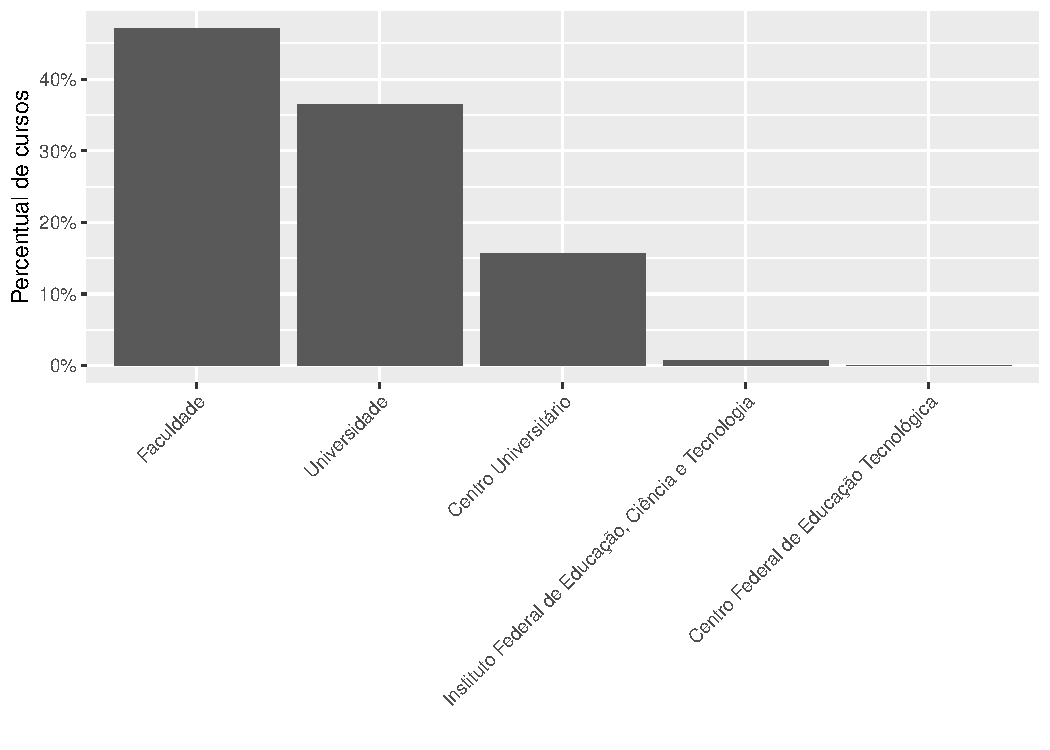
\includegraphics[scale=.90]{../../graficos/latex-graph-percent-de-cursos-p-org-acad.pdf}
		\caption{Percentual de cursos por organização acadêmica}
		\label{fig: graf-percent-cursos-org-acad}
	\end{figure}
	\pagebreak
	\item \textbf{Percentual de cursos por Categoria Administrativa}:
	\begin{figure}[H]
		\centering
		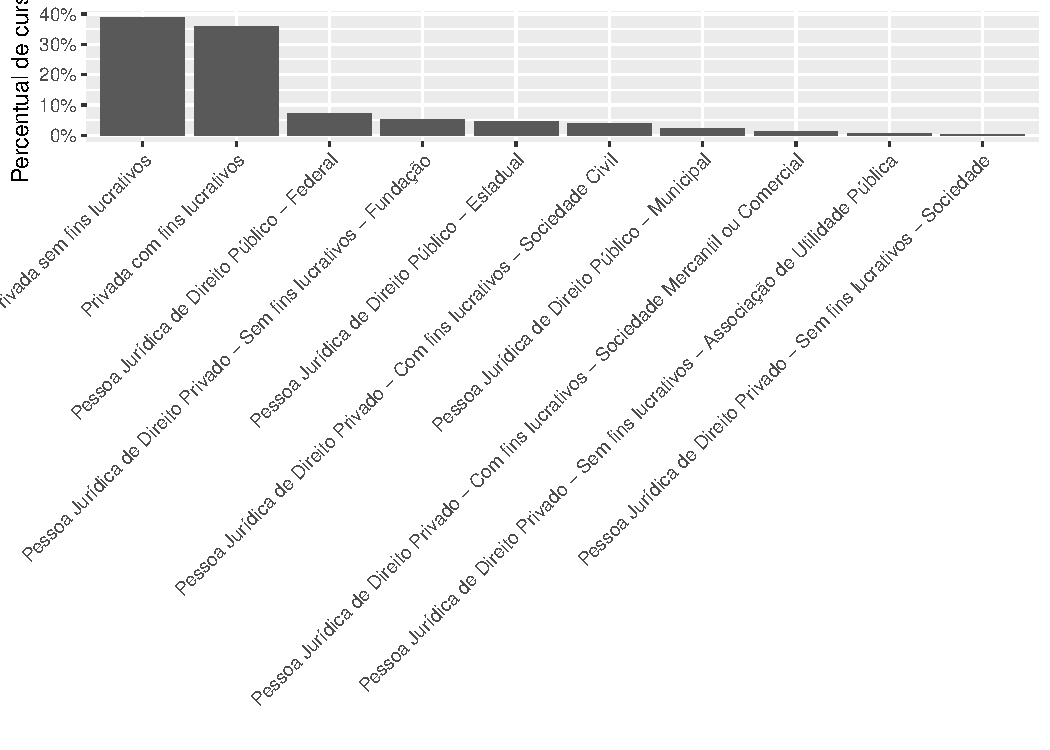
\includegraphics[scale=.9]{../../graficos/latex-graph-percent-de-cursos-p-cat-adm.pdf}
		\caption{Percentual de cursos por categoria administrativa}
		\label{fig: graf-percent-cursos-cat-adm}
	\end{figure}
	\item \textbf{IES por categoria administrativa}:
	% Please add the following required packages to your document preamble:
% \usepackage{booktabs}
% \usepackage{graphicx}
\begin{table}[H]
\centering
\resizebox{\textwidth}{!}{%
\begin{tabular}{@{}ll@{}}
\toprule
\textbf{Categoria Administrativa}                                                           & \textbf{Total} \\ \midrule
Privada com fins lucrativos                                                                 & 681            \\
Privada sem fins lucrativos                                                                 & 671            \\
Pessoa Jurídica de Direito Privado - Sem fins lucrativos - Fundação                         & 94             \\
Pessoa Jurídica de Direito Público - Federal                                                & 91             \\
Pessoa Jurídica de Direito Privado - Com fins lucrativos - Sociedade Civil                  & 70             \\
Pessoa Jurídica de Direito Público - Estadual                                               & 68             \\
Pessoa Jurídica de Direito Público - Municipal                                              & 43             \\
Pessoa Jurídica de Direito Privado - Com fins lucrativos - Sociedade Mercantil ou Comercial & 25             \\
Pessoa Jurídica de Direito Privado - Sem fins lucrativos - Associação de Utilidade Pública  & 9              \\
Pessoa Jurídica de Direito Privado - Sem fins lucrativos - Sociedade                        & 6              \\ \bottomrule
\end{tabular}%
}
\end{table}

	\item \textbf{Variável resposta}: Conceito Preliminar de Curso. Sobre a variável resposta \textit{CPC Faixa} foi observado que 12,97\% dos cursos não obtiveram notas\footnotemark. Os demais cursos estão relacionados na figura \ref{graf: cursos-com-conceito} e na tabela \ref{tbl: cursos-com-conceito}:
	\footnotetext{Cursos não reconhecidos: 847 (10.4\%);
	Cursos sem conceito: 205 (2.52\%);
	Cursos sub judice: 2 (0.0246\%)}

	\begin{figure}[H]
		\centering
		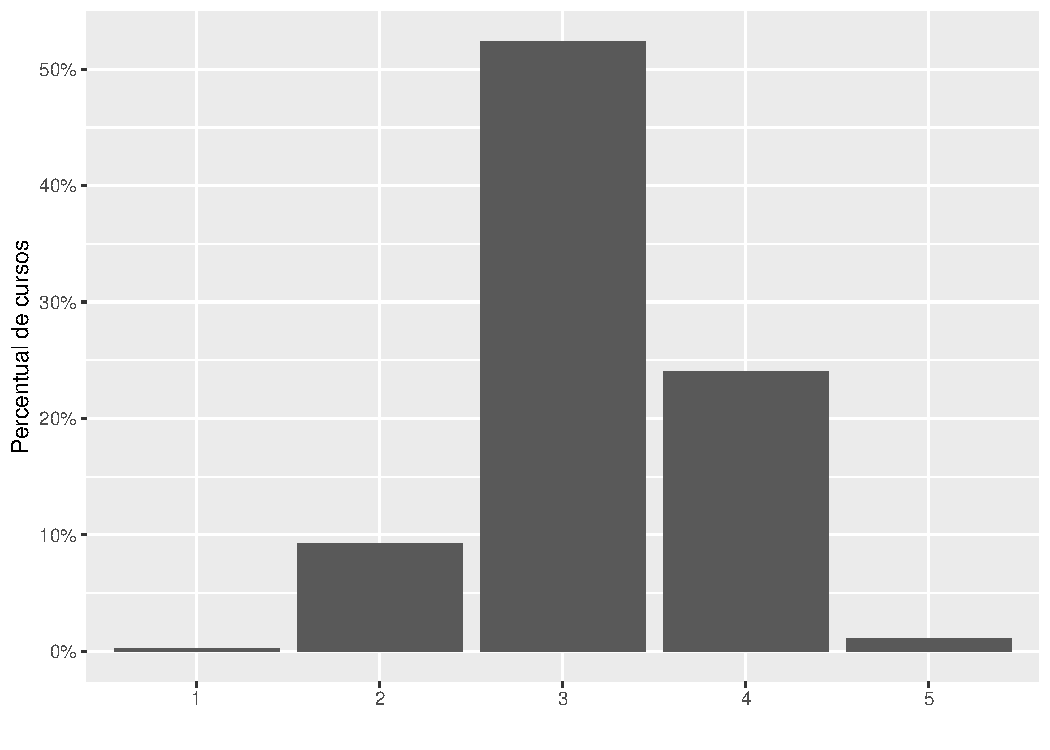
\includegraphics[scale=.75]{../../graficos/latex-graph-cursos-com-conceito.pdf}
		\caption{Cursos com conceito}
		\label{graf: cursos-com-conceito}
	\end{figure}

	% Please add the following required packages to your document preamble:
% \usepackage{booktabs}
\begin{table}[H]
\centering
\begin{tabular}{@{}lll@{}}
\toprule
\textbf{Conceito} & \textbf{Frequência} & \textbf{Percentual} \\ \midrule
1                 & 22                  & 0.3\%               \\
2                 & 753                 & 9.3\%               \\
3                 & 4252                & 52.4\%              \\
4                 & 1949                & 24.0\%              \\
5                 & 91                  & 1.1\%               \\ \bottomrule
\end{tabular}
\caption{Cursos com conceito}
\label{tbl: cursos-com-conceito}
\end{table}

	\item \textbf{Análise das variáveis numéricas}: Sabe-se que alguns cursos não obtiveram conceito pelo fato de estarem na condição de não reconhecidos, sem conceito ou sub judice. Foi observado, contudo que tais cursos apesar de estarem com o campo CPC Faixa vazios (e portanto sem a principal variável, a de resposta), tiveram notas nas variáveis preditoras. A partir desta constatação foi possível concluir que a utilização dessas observações nas modelagens estatísticas traria prejuízos significativos em termos de precisão.

	Com a finalidade de minimizar os efeitos da influência de observações vazias, duas abordagens foram inicialmente estudadas. A primeira consiste em utilizar o método de imputação de dados denominado $k$-NN\footnote{Este método encontra-se implementado no pacote \lstinline{DMwR} sob autoria de \citeonline{DMwR}.}~(\textit{k-Nearest Neighbors algorithm}) procura estimar o valor da observação vazia a partir de um parâmetro $k$ que representa a distância deste aos seus $k$ vizinhos mais próximos.

	Na segunda abordagem foram omitidas as observações vazias sob a hipótese de que as mesmas estão suficientemente representadas pelas demais observações. Desta forma a criação de um modelo não perderia eficiência nem estaria enviesado. A tabela \ref{tbl: sumario-estatisico-com-knn} contém a sumarização estatística das variáveis preditoras. Nela foi utilizada a técnica de estimação das observações vazias pelo método $k$-NN. Não foram verificadas diferenças significativas nas medidas estatísticas que implicassem em impossibilidade de estimação pelo método proposto.

	Como \citeonline[p.~2]{josse2016missmda} de forma bem elucidativa aborda, manipular bases com dados faltantes utilizando PCA pode ser uma tarefa complicada pela limitação que alguns softwares têm em gerar resultados a partir de campos vazios. Segundo esse autor a aplicação do método $k$-NN pressupõe que as variáveis estejam sob distribuição Gaussiana e é seguramente um método de imputação de variáveis contínuas bastante popular \Ibidem[p.~24]{josse2016missmda}. A sumarização estatística utilizando o método pode ser vista na tabela \ref{tbl: sumario-estatisico-com-knn}.

	% Please add the following required packages to your document preamble:
% \usepackage{booktabs}
% \usepackage{graphicx}
\begin{table}[H]
\centering
\resizebox{\textwidth}{!}{%
\begin{tabular}{@{}llllllll@{}}
\toprule
\textbf{Variável}                                         & \textbf{Média} & \textbf{Desvio padrão} & \textbf{Mediana} & \textbf{Moda} & \textbf{Mínimo} & \textbf{Máximo} & \textbf{n} \\ \midrule
Concluintes Inscritos                                     & 67.6625        & 204.194                & 39               & 25            & 1               & 11155           & 8121       \\
Concluintes Participantes                                 & 55.0494        & 162.6907               & 32               & 20            & 0               & 10059           & 8121       \\
Nota Bruta - FG                                           & 54.1955        & 6.2626                 & 53.8867          & 55.8          & 4.7127          & 80.65           & 8121       \\
Nota Bruta - CE                                           & 42.5299        & 8.228                  & 41.46            & 44.6          & 4.1746          & 80.8091         & 8121       \\
Nota Bruta - Geral                                        & 45.4587        & 7.0596                 & 44.7091          & 47.6          & 4.3141          & 79.75           & 8121       \\
Nota Contínua do Enade                                    & 2.3915         & 0.8577                 & 2.324            & 5             & 0               & 5               & 8121       \\
Nota Bruta - Organização Didático-Pedagógica              & 5.2105         & 0.481                  & 5.221            & 6             & 1.7121          & 6               & 8121       \\
Nota Padronizada - Organização Didático-Pedagógica        & 3.0204         & 1.1832                 & 3.0213           & 5             & 0               & 5               & 8121       \\
Nota Bruta - Infraestrutura e Instalações Físicas         & 4.9685         & 0.6723                 & 5.0136           & 6             & 2               & 6               & 8121       \\
Nota Padronizada - Infraestrutura e Instalações Físicas   & 3.1313         & 1.2076                 & 3.1954           & 5             & 0               & 5               & 8121       \\
Nota Bruta - Oportunidades de Ampliação da Formação       & 4.5659         & 0.8142                 & 4.5565           & 6             & 1.1905          & 6               & 8121       \\
Nota Padronizada - Oportunidades de Ampliação da Formação & 2.9541         & 1.1725                 & 2.9522           & 5             & 0               & 5               & 8121       \\
Concluintes Participantes com nota no Enem                & 28.7791        & 67.3562                & 17               & 7             & 1               & 3842            & 8121       \\
Percentual de Concluintes participantes com nota no Enem  & 0.5344         & 0.206                  & 0.5385           & 0.5           & 0.0143          & 1               & 8121       \\
Nota Bruta - IDD                                          & -0.1043        & 2.3789                 & -0.0948          & -1.5685       & -23.6519        & 24.4723         & 8121       \\
Nota Padronizada - IDD                                    & 2.4782         & 0.8428                 & 2.4758           & 0             & 0               & 5               & 8121       \\
Nr. de Docentes                                           & 26.1061        & 21.6867                & 20               & 16            & 0               & 298             & 8121       \\
Nota Bruta - Mestres                                      & 0.7633         & 0.2083                 & 0.8077           & 1             & 0               & 1               & 8121       \\
Nota Padronizada - Mestres                                & 3.5552         & 1.2234                 & 3.7796           & 5             & 0               & 5               & 8121       \\
Nota Bruta - Doutores                                     & 0.3124         & 0.2219                 & 0.2766           & 0             & 0               & 1               & 8121       \\
Nota Padronizada - Doutores                               & 1.7291         & 1.2051                 & 1.5541           & 0             & 0               & 5               & 8121       \\
Nota Bruta - Regime de Trabalho                           & 0.7592         & 0.238                  & 0.8125           & 1             & 0               & 1               & 8121       \\
Nota Padronizada - Regime de Trabalho                     & 3.6919         & 1.2766                 & 3.9688           & 5             & 0               & 5               & 8121       \\
CPC Contínuo                                              & 2.6111         & 0.5807                 & 2.609            & 1.0491        & 0.4257          & 4.6885          & 8121       \\
CPC Faixa                                                 & 3.1711         & 0.6371                 & 3                & 3             & 1               & 5               & 8121       \\ \bottomrule
\end{tabular}%
}
\caption{Sumarização da base de dados após uso do método $k$-NN: medidas estatísticas básicas}
\label{tbl: sumario-estatisico-com-knn}
\end{table}
	\end{enumerate}
\pagebreak

